% Copyright 2022 by Sébastien Descotes-Genon
%
% This file may be distributed and/or modified
%
% 1. under the LaTeX Project Public License and/or
% 2. under the GNU Public License.
%


\documentclass{beamer}

\usepackage{array,amsmath}
\newcolumntype{L}{>$l<$}



% Setup appearance:

\usetheme{IJCLab}

\pgfdeclareimage[height=2cm]{LogoIJCLab}{example-fig/LogoIJCLab}
\pgfdeclareimage[height=1.3cm]{LogoCNRS}{example-fig/LogoCNRS}
\pgfdeclareimage[height=1cm]{LogoUPSay}{example-fig/LogoUPSay}


\usepackage[english]{babel}
\usepackage[T1]{fontenc}


% Author, Title, etc.

\title[Atmospheric transparency at LSST Obs]{\large Photometric Calibration at Rubin-LSST observatory \\
Estimation of atmospheric transparency \\ Correction for Water \& Aerosol variations\\
{\small Univers du Pôle A2C}}

\titlegraphic{\begin{center}\qquad\pgfuseimage{LogoCNRS}\qquad\quad\qquad\quad\pgfuseimage{LogoIJCLab}\qquad\qquad\pgfuseimage{LogoUPSay}\end{center}}

\author[S. Dagoret-Campagne]{
Sylvie Dagoret-Campagne,Marc Moniez, Martin Rodriguez Monroy, Joseph Chevalier,
Jeremy Neveu
}
\institute[IJCLab]{
  IJCLab,
  CNRS/IN2P3 \& Université Paris-Saclay,
  Orsay, France }
  
  % Caution  : This is not the affiliation to be used to sign articles. 
  % Please refer to the intranet : Bibliothèque/IST / Règles de publication
     
\date[IJCLab, Dec 14th 2022]{IJCLab, pôle A2C, December 14th 2022}


% The main document with a few examples

\begin{document}

%==================================================================================================================================
\begin{frame}
  \titlepage
\end{frame}
%==================================================================================================================================



\begin{frame}
\begin{columns}[T] % align columns
\begin{column}{.48\textwidth}
\color{red}\rule{\linewidth}{4pt}

\begin{eqnarray}
m_b^{std} & = &  -2.5 \log_{10}(C_b^{obs}) \nonumber \\ 
& & + 2.5 \log_{10}\left(\mathbb{I}_0^{obs}(b)\right) \nonumber \\
& & + ZPT^{AB}   \nonumber \\
& & + 2.5 \log_{10} 
	\left( 
	\frac{\int_0^\infty F_\nu(\lambda) \times \phi_b^{obs}(\lambda) d\lambda }{\int_0^\infty F_\nu(\lambda) \times \phi_b^{std}(\lambda) d\lambda} 
	\right)
\end{eqnarray}


\end{column}%
\hfill%
\begin{column}{.48\textwidth}
\color{blue}\rule{\linewidth}{4pt}

Right Part
\end{column}%
\end{columns}
\end{frame}


\begin{frame}

$$
\begin{array}{lcl c r}
m_b^{std} & = &  -2.5 \log_{10}(ADU_b^{obs}) & \longrightarrow &  \\ 
& & + 2.5 \log_{10}\left(\mathbb{I}_0^{obs}(b)\right) & \longrightarrow \\
& & + ZPT^{AB}   \nonumber \\
& & + 2.5 \log_{10} 
	\left( 
	\frac{\int_0^\infty F_\nu(\lambda) \times \phi_b^{obs}(\lambda) d\lambda }{\int_0^\infty F_\nu(\lambda) \times \phi_b^{std}(\lambda) d\lambda} 
	\right)
\end{array}
$$
\end{frame}

% see example https://tex.stackexchange.com/questions/62902/text-column-in-array
% Define a text column environnement
%\usepackage{array,amsmath}
%\newcolumntype{L}{>$l<$}

%\begin{frame}
%\begin{equation*}
%    \begin{array}{L@{\quad}c@{{}={}}c}
%       some text:            & x^2 & x^2 \\
%       more thoughts:        & y^2 & y^2 \\
%       really deep thoughts: & z^2 & z^2
%    \end{array}
%\end{equation*}
%\end{frame}


\begin{frame}{Magnitude calibration of astronomical objects}
\begin{alertblock}{Single visit object magnitude to be coadded in band $b$}
\begin{equation*}
    \begin{array}{l@{{}{}}c c@{\quad}L}
               m_b^{std} =   & -2.5 \log_{10}(ADU_b^{obs}) & \longrightarrow  & ADU photometric counts     \\
                & +  2.5 \log_{10}\left(\mathbb{I}_0^{obs}(b)\right)  &\longrightarrow  &  {\color{red}0th order transmission term} \\
                 & + ZPT^{AB}_{obs}  & \longrightarrow & Zero Point magnitude \\
                 &  +  2.5 \log_{10} 
	\left( 
	\frac{\int_0^\infty F_\nu(\lambda) \times \phi_b^{obs}(\lambda) d\lambda }{\int_0^\infty F_\nu(\lambda) \times \phi_b^{std}(\lambda) d\lambda} 
	\right) & \longrightarrow & {\color{blue}SED Color correction term}
    \end{array}
\end{equation*}
\end{alertblock}
{\footnotesize
\begin{block}{Calibration quantities for each observation:}
\begin{equation*}
\begin{array}{L@{\quad}ccc}
transmission integral : & \mathbb{I}_0^{obs}(b) & \equiv & \int_0^\infty S^{obs}_b(\lambda) \frac{d\lambda}{\lambda} \\
zero point link to AB-flux unit/CCD : & ZPT^{AB}_{obs} & \equiv & 2.5 \log_{10} \left( \frac{A \Delta T F^{AB}}{gh}\right)
\end{array} 
\end{equation*}
\end{block}
\begin{itemize}
\item Total transmission : $S_b^{obs}(\lambda) = S^{atm}(\lambda) \times S_b^{inst}(\lambda)$
\item Normalized passband : $\phi_b^{obs} (\lambda,t) = \frac{S_b^{obs}(\lambda,t)\frac{1}{\lambda}}{\int_0^\infty S^{obs}_b(\lambda,t) \frac{d\lambda}{\lambda}}$
\end{itemize}
}
\end{frame}


%==================================================================================================================================
\begin{frame}{Motivations}
\begin{itemize}
\item Sources/Object standard magnitude estimation from instrumental magnitude $\rightarrow$ allowing coaddition of sigle epoch measurements
\item use of time dependent epoch transmissions (instrument + atmosphere)
\item photometric correction depending on poorly known objects SED
\item to be implemented inside DM Rubin-LSST science pipelines 
\item participation of DESC technical groups (SAWG,PCWG,PSF), namely during commissioning phase,
\item need participation of Science groups (PhotoZ, and objects groups like SN, and other astrophysical groups),
\end{itemize}
\end{frame}
%==================================================================================================================================

%==================================================================================================================================
\begin{frame}{Outline}
  \tableofcontents
\end{frame}
%==================================================================================================================================




\section{Key formula, definitions and notations}
\subsection{Instrumental Flux}

%==================================================================================================================================
\begin{frame}{Instrumental Flux}
\begin{alertblock}{Photometric flux of a source}
	\begin{equation}
	ADU_b = \frac{A\Delta T}{gh}\int_0^\infty F_\nu(\lambda) \times S_b^{obs}(\lambda,x,y,az,alt,t) \frac{d\lambda}{\lambda}
	\end{equation}
	\begin{itemize}
	\item $ADU_b$ : ADU count of a source measured by photometry in band $b$
	\item $F_\nu$ : SED in ${\rm erg/cm^2/Hz/s}$
	\item $S_b^{obs}$ : Observation transmission in band $b$(atmosphere + instrument)
	\item $A$ : Collection efficiency in ${\rm cm^2}$
	\item $g$ : Electronic gain in ${\rm e^-/ADU}$
	\item $\Delta T$ : Exposure time
	\item $h$ : Planck constant
	\end{itemize}
	\end{alertblock}	
\end{frame}
%=================================================================================================================================


\subsection{Observed Magnitude}
%=================================================================================================================================
\begin{frame}{Observed Magnitude}
\begin{alertblock}{Observed Magnitude of a source}
	\begin{equation}
	m^{obs}_b = -2.5 \log_{10}\left( 
	\frac{\int_0^\infty F_\nu(\lambda) \times S_b^{obs}(\lambda,x,y,az,alt,t) \frac{d\lambda}{\lambda} }{\int_0^\infty F^{AB} \times S_b^{obs}(\lambda,x,y,az,alt,t) \frac{d\lambda}{\lambda}} 
	\right)
	\end{equation}
	\begin{itemize}
	\item $m^{obs}_b$ : observed magnitude in band $b$
	\item $F_\nu$ : SED in ${\rm erg/cm^2/Hz/s}$
	\item $F^{AB}=3631 Jy$ : Flat SED with $1 Jy = 10^{-23} {\rm erg/cm^2/Hz/s}$
	\item $S_b^{obs}$ : Observation transmission in band $b$  (atmosphere + instrument)
	\end{itemize}
	\end{alertblock}	
In the above formula gives how the physics provides $m_b^{obs}$. However usually the $F_\nu(\lambda)$ of an object is unknown.	
Note $m^{obs}_b$ is defined independently of any reference to a standard magnitude.
\end{frame}
%========================================================================================================================



%========================================================================================================================
\begin{frame}{Natural magnitude in Rubin-LSST}
Rubin-LSST usually use the concept of normalized passband
\begin{alertblock}{normalized bandpass response function}
\begin{equation}
\phi_b^{obs} (\lambda,t) = \frac{S_b^{obs}(\lambda,t)\frac{1}{\lambda}}{\int_0^\infty S^{obs}_b(\lambda,t) \frac{d\lambda}{\lambda}}
\end{equation}
\end{alertblock}
\begin{block}{Observed flux}
\begin{equation}
F_b^{obs} = \int_0^\infty F_\nu(\lambda) \phi_b^{obs}(\lambda) d\lambda
\end{equation}
\end{block}
\begin{exampleblock}{Natural magnitude}
\begin{equation}
m_b^{nat} = -2.5 \log_{10} \left( \frac{F_b^{obs}}{F^{AB}}\right)
\end{equation}
\end{exampleblock}
The natural magnitude $m_b^{nat}$ is similar to  the observed magnitude $m_b^{obs}$
\end{frame}
%=========================================================================================================================



%========================================================================================================================
\begin{frame}{Decomposition of observed Magnitude} 
The observed magnitude is estimated from the measured ADU counts rate $C_b=ADU_b/\Delta T$ in filter $b$
\begin{alertblock}{}
\begin{equation}
m^{obs}_b = -2.5 \log_{10}(C_b)+ 2.5 \log_{10}\left(\mathbb{I}_0^{obs}(b)\right) + ZPT^{AB}
\end{equation}	
\end{alertblock}	
However the two following quantities which depend on atmospheric + detectors conditions must be estimated by calibration. 
\begin{block}{Calibration quantities:}
\begin{eqnarray}
\mathbb{I}_0^{obs}(b) & \equiv & \int_0^\infty S^{obs}_b(\lambda) \frac{d\lambda}{\lambda} \\
ZPT^{AB} & \equiv & 2.5 \log_{10} \left( \frac{A F^{AB}}{gh}\right)
\end{eqnarray} 
\end{block}

\end{frame}
%==========================================================================================================================

%==========================================================================================================================
\begin{frame}{Zero point} 
Note sometimes one defines the zero point as the magnitude $m_b^{obs}$, such $ADU_b/\Delta T = 1$ count per sec, then
\begin{equation}
m^{obs}_b(ZP) \equiv 2.5\log_{10}\left( \mathbb{I}_0^{obs}(b)\right) + ZPT^{AB}
\end{equation}	
\begin{itemize}
\item the zero point is common to all sources whatever their color is 
\item it has a time  dependent and passband $b$ dependent component : $2.5\log_{10}\left( \mathbb{I}_0^{obs}(b)\right)$
\item it has a detector (CCD) dependent component :  $ZPT^{AB}$ through the relative electronic gain $g$, (independent of the passband $b$ ?, long time-scale dependence (night) ?)
\end{itemize}
\end{frame}
%==========================================================================================================================



\subsection{Standard Magnitude}
%==========================================================================================================================
\begin{frame}{Standard Magnitude} 
Standard magnitude is the magnitude to be published with the standard passband. 
It must be calculated from the observed magnitude.
\begin{alertblock}{Standard magnitude in standard passband}
	\begin{equation}
	m^{std}_b = -2.5 \log_{10}
	\left( 
	\frac{\int_0^\infty F_\nu(\lambda) \times S_b^{std}(\lambda) \frac{d\lambda}{\lambda} }{\int_0^\infty F^{AB} \times S_b^{std}(\lambda) \frac{d\lambda}{\lambda}} 
	\right)
	\end{equation}	
\end{alertblock}	

\begin{eqnarray}
\delta^{std}_b & \equiv & m_b^{std} - m_b^{obs} \\
& \equiv & 2.5 \log_{10}\left( \frac{\mathbb{I}_0^{std}(b)}{\mathbb{I}_0^{obs}(b)}\right) 
+ 2.5 \log_{10} 
	\left( 
	\frac{\int_0^\infty F_\nu(\lambda) \times S_b^{obs}(\lambda) \frac{d\lambda}{\lambda} }{\int_0^\infty F_\nu(\lambda) \times S_b^{std}(\lambda) \frac{d\lambda}{\lambda}} 
	\right)
\end{eqnarray} 
\end{frame}
%==========================================================================================================================

%==========================================================================================================================
\begin{frame}{Standard magnitude in Rubin-LSST}
\begin{alertblock}{standard magnitude}
\begin{eqnarray}
m_b^{std} & = & m_b^{nat} + \Delta m_b^{obs} \\
\Delta m_b^{obs} & = & 2.5 \log_{10} \frac{\int_0^\infty F_\nu(\lambda) \phi_b^{obs}(\lambda) d\lambda}{\int_0^\infty F_\nu(\lambda) \phi_b^{std}(\lambda) d\lambda}
\end{eqnarray}
\end{alertblock}
\begin{block}{}
{\small
\begin{eqnarray}
\Delta m_b^{obs} = \delta_b^{std} & = & 2.5 \log_{10}\left( \frac{\mathbb{I}_0^{std}(b)}{\mathbb{I}_0^{obs}(b)}\right) 
+ 2.5 \log_{10} 
	\left( 
	\frac{\int_0^\infty F_\nu(\lambda) \times S_b^{obs}(\lambda) \frac{d\lambda}{\lambda} }{\int_0^\infty F_\nu(\lambda) \times S_b^{std}(\lambda) \frac{d\lambda}{\lambda}} 
	\right) \nonumber \\
& = & 	2.5 \log_{10} 
	\left( 
	\frac{\int_0^\infty F_\nu(\lambda) \times \phi_b^{obs}(\lambda) d\lambda}{\int_0^\infty F_\nu(\lambda) \times \phi_b^{std}(\lambda) d\lambda} 
	\right) \nonumber	
\end{eqnarray}
}
\end{block}
\end{frame}
%==========================================================================================================================




%==========================================================================================================================
\begin{frame}{Zero Point in Rubin-LSST}
\begin{exampleblock}{Zero point definition}
\begin{eqnarray}
m_b^{std} & = & -2.5 \log_{10}(C_b^{obs}) + \Delta m_b^{obs} + Z_b^{obs}
\end{eqnarray}
with $C_b^{obs} = ADU_b/\Delta T$
\end{exampleblock}
\begin{alertblock}{Correspondence of Zero point in Rubin-DES}
\begin{equation}
Z_b^{obs} = 2.5\log_{10}\left(\mathbb{I}_0^{obs}(b)\right) + ZPT^{AB}
\end{equation}
\end{alertblock}
\end{frame}
%==========================================================================================================================


%==========================================================================================================================
\begin{frame}{Interpretable standard magnitude expression}
\begin{alertblock}{option A : with zero point as unit counting rate}
\begin{eqnarray}
m_b^{std} & = &  -2.5 \log_{10}(C_b^{obs})+ 2.5 \log_{10}\left(\frac{\mathbb{I}_0^{std}(b)}{\mathbb{I}_0^{obs}}\right) + m_b^{obs}(ZPT)   \nonumber \\
 & & + 2.5 \log_{10} 
	\left( 
	\frac{\int_0^\infty F_\nu(\lambda) \times S_b^{obs}(\lambda) \frac{d\lambda}{\lambda} }{\int_0^\infty F_\nu(\lambda) \times S_b^{std}(\lambda) \frac{d\lambda}{\lambda}} 
	\right)
\end{eqnarray}
\end{alertblock}
\begin{itemize}
\item $-2.5 \log_{10}(C_b^{obs})$ : measured instrumnetal aperture photometric term (ADU rate)
\item $2.5 \log_{10}\left(\frac{\mathbb{I}_0^{std}(b)}{\mathbb{I}_0^{obs}}\right)$ : SED color free correction term for atmospheric transparency standard/observed
\item $m_b^{obs}(ZPT)$ :  SED color free observed magnitude Zero Point correction term at CCD level,
\item $2.5 \log_{10} 
	\left( 
	\frac{\int_0^\infty F_\nu(\lambda) \times S_b^{obs}(\lambda) \frac{d\lambda}{\lambda} }{\int_0^\infty F_\nu(\lambda) \times S_b^{std}(\lambda) \frac{d\lambda}{\lambda}}\right)$ : SED color dependent term correction
\end{itemize}
\end{frame}
%============================================================================================




%==========================================================================================================================
\begin{frame}{Interpretable standard magnitude expression}
\begin{alertblock}{option B : with zero point as constants}
\begin{eqnarray}
m_b^{std} & = &  -2.5 \log_{10}(C_b^{obs})+ 2.5 \log_{10}\left(\mathbb{I}_0^{std}(b)\right) + ZPT^{AB}   \nonumber \\
 & & + 2.5 \log_{10} 
	\left( 
	\frac{\int_0^\infty F_\nu(\lambda) \times S_b^{obs}(\lambda) \frac{d\lambda}{\lambda} }{\int_0^\infty F_\nu(\lambda) \times S_b^{std}(\lambda) \frac{d\lambda}{\lambda}} 
	\right)
\end{eqnarray}
\end{alertblock}
\begin{itemize}
\item $-2.5 \log_{10}(C_b^{obs})$ : measured instrumental aperture photometric term (ADU rate)
\item $2.5 \log_{10}\left(\mathbb{I}_0^{std}(b)\right)$ : Calculable constant
\item $ZPT^{AB} = \frac{A F^{AB}}{gh}$ :  SED color free observed magnitude Zero Point correction term at CCD level (electronic gain),
\item $2.5 \log_{10} 
	\left( 
	\frac{\int_0^\infty F_\nu(\lambda) \times S_b^{obs}(\lambda) \frac{d\lambda}{\lambda} }{\int_0^\infty F_\nu(\lambda) \times S_b^{std}(\lambda) \frac{d\lambda}{\lambda}}\right)$ : SED color dependent term correction
\end{itemize}
\end{frame}
%============================================================================================



%==========================================================================================================================
\begin{frame}{Interpretable standard magnitude expression}
\begin{alertblock}{option C : using normalized passband}
\begin{eqnarray}
m_b^{std} & = &  -2.5 \log_{10}(C_b^{obs})+ 2.5 \log_{10}\left(\mathbb{I}_0^{obs}(b)\right) + ZPT^{AB}   \nonumber \\
 & & + 2.5 \log_{10} 
	\left( 
	\frac{\int_0^\infty F_\nu(\lambda) \times \phi_b^{obs}(\lambda) d\lambda }{\int_0^\infty F_\nu(\lambda) \times \phi_b^{std}(\lambda) d\lambda} 
	\right)
\end{eqnarray}
\end{alertblock}
\begin{itemize}
\item $-2.5 \log_{10}(C_b^{obs})$ : measured instrumental aperture photometric term (ADU rate)
\item $2.5 \log_{10}\left(\mathbb{I}_0^{obs}(b)\right)$ : order 0 correction : measured variable absorption in the band $b$ (compensate $C_b^{obs}$)
\item $ZPT^{AB} = \frac{A F^{AB}}{gh}$ :  SED color free observed magnitude Zero Point correction term at CCD level (electronic gain),
\item $2.5 \log_{10} 
	\left( 
	\frac{\int_0^\infty F_\nu(\lambda) \times \phi_b^{obs}(\lambda) d\lambda}{\int_0^\infty F_\nu(\lambda) \times \phi_b^{std}(\lambda) d\lambda}\right)$ : SED color dependent term correction
\end{itemize}
\end{frame}
%============================================================================================




\subsection{Approximation for SED shape}
%==========================================================================================================================
\begin{frame}{Approximation for SED shape} 
\begin{exampleblock}{SED approximation as Taylor expansion}
\begin{eqnarray}
F_\nu(\lambda) & = & F_\nu(\lambda_b) \left(1 + f^\prime(\lambda_b)(\lambda-\lambda_b) + \frac{f^{\prime\prime}(\lambda_b)}{2}(\lambda-\lambda_b)^2 + \cdots \right) \\
f_\nu^\prime(\lambda) & \equiv & \frac{1}{F_\nu(\lambda)}\frac{dF_\nu(\lambda)}{d\lambda} \qquad \qquad \qquad
f_\nu^{\prime\prime}(\lambda)  \equiv  \frac{1}{F_\nu(\lambda)}\frac{d^2F_\nu(\lambda)}{d\lambda^2} \nonumber \\
\lambda_b & \equiv & \frac{\int_0^{\infty} \lambda \times S_b^{inst}(\lambda) \frac{d\lambda}{\lambda}}
{\int_0^{\infty} S_b^{inst}(\lambda) \frac{d\lambda}{\lambda}}
\end{eqnarray}
\begin{itemize}
\item $S_b^{obs}(\lambda) = S_b^{inst}(\lambda,t,x,y) \times S^{atm}(\lambda,t,alt,az)$
\end{itemize}
\end{exampleblock}
\end{frame}
%==========================================================================================================================

\subsection{Summary of definitions on interpretable standard magnitude}
%==========================================================================================================================
\begin{frame}{Summary of definitions}
\begin{alertblock}{Decomposition of standard magnitude}
\begin{eqnarray}
m_b^{std} & = & -2.5 \log_{10}(C_b)  \nonumber \\
          &   &  + 2.5 \log_{10}(\mathbb{I}_0^{obs}(b)) + ZPT^{AB}  \nonumber \\
          &   &  + 2.5 \log_{10}\left( 
\frac{1 + f_\nu^\prime(\lambda_b)\mathbb{I}^{obs}_{10}(b)  +\frac{f_\nu^{\prime\prime}(\lambda_b)}{2}\mathbb{I}_{20}^{obs}(b)}
{1 + f_\nu^\prime(\lambda_b)\mathbb{I}^{std}_{10}(b)  +\frac{f_\nu^{\prime\prime}(\lambda_b)}{2}\mathbb{I}_{20}^{std}(b)}\right)
\end{eqnarray}
\end{alertblock}
\end{frame}
%==========================================================================================================================


%==========================================================================================================================
\begin{frame}{Transmission moments definitions}
\begin{block}{Transmission moments definitions}

\begin{eqnarray}
\mathbb{I}_0^i(b) & = & \int_0^{\infty} S_b^i(\lambda) \frac{d\lambda}{\lambda} \\
\mathbb{I}_1^i(b) & = & \int_0^{\infty} (\lambda-\lambda_b) S_b^i(\lambda) \frac{d\lambda}{\lambda} \\
 \mathbb{I}_2^i(b) & = &\int_0^{\infty} (\lambda-\lambda_b)^2 S_b^i(\lambda) \frac{d\lambda}{\lambda} \\
\mathbb{I}^i_{10}(b)  & = &\frac{\mathbb{I}^i_1(b)}{\mathbb{I}^i_0(b)} \\
\mathbb{I}^i_{20}(b) & = & \frac{\mathbb{I}^i_2(b)}{\mathbb{I}^i_0(b)} 
\end{eqnarray}

with $i=obs$ or $i=std$
\end{block}
\end{frame}
%==========================================================================================================================




\subsection{SED shape correction}
%==========================================================================================================================
\begin{frame}{Approximation for SED shape correction}
\begin{alertblock}{SED shape ($f^\prime_\nu,f^{\prime\prime}_\nu$) color correction}
\begin{eqnarray}
m_b^{std} & = & -2.5 \log_{10}(C_b)  \nonumber \\
          &   &  + 2.5 \log_{10}(\mathbb{I}_0^{obs}(b)) + ZPT^{AB}  \nonumber \\
          &   &  + 1.087\left( f_\nu^\prime(\lambda_b) \Delta \mathbb{I}_{10}(b) +
          \frac{f_\nu^{\prime\prime}(\lambda_b)}{2}\Delta \mathbb{I}_{20}(b) \right. \nonumber \\
         & & - \left. \frac{1}{2}\left( f_\nu^\prime(\lambda_b) \Delta \mathbb{I}_{10}(b) \right)^2             
          \right)
\end{eqnarray}
\end{alertblock}
\begin{block}{Moments difference definition}
\begin{eqnarray}
\Delta \mathbb{I}_{10}(b) & = &  \mathbb{I}_{10}^{obs}(b)  -  \mathbb{I}_{10}^{std}(b) \\
\Delta \mathbb{I}_{20}(b) & = &   \mathbb{I}_{20}^{obs}(b)  -  \mathbb{I}_{20}^{std}(b) 
\end{eqnarray}
\end{block}
\end{frame}
%==========================================================================================================================



\subsection{Bias on Magnitude for SED shape correction}
%==========================================================================================================================
\begin{frame}{Bias on Magnitude for SED shape correction}
\begin{alertblock}{Error on Magnitude for SED-shape correction}
\begin{eqnarray}
\Delta m & = & \left| 2.5 \log_{10}\left(
\frac{\mathbb{I}_0^{std}(b)}
{\mathbb{I}_0^{obs}(b)}\right) +
2.5 \log_{10} 
	\left( 
	\frac{\int_0^\infty F_\nu(\lambda) \times S_b^{obs}(\lambda) \frac{d\lambda}{\lambda} }{\int_0^\infty F_\nu(\lambda) \times S_b^{std}(\lambda) \frac{d\lambda}{\lambda}} 
	\right) \right. \nonumber \\
    & & \left. - 1.087\left( f_\nu^\prime(\lambda_b) \Delta \mathbb{I}_{10}(b) +
          \frac{f_\nu^{\prime\prime}(\lambda_b)}{2}\Delta \mathbb{I}_{20}(b) \right. 
         - \left. \frac{1}{2}\left( f_\nu^\prime(\lambda_b) \Delta \mathbb{I}_{10}(b) \right)^2             
          \right)\right| \nonumber \\
\Delta m & = & \left| 
2.5 \log_{10} 
	\left( 
	\frac{\int_0^\infty F_\nu(\lambda) \times \phi_b^{obs}(\lambda) d\lambda}{\int_0^\infty F_\nu(\lambda) \times \phi_b^{std}(\lambda)d\lambda} 
	\right) \right. \nonumber \\
    & & \left. - 1.087\left( f_\nu^\prime(\lambda_b) \Delta \mathbb{I}_{10}(b) +
          \frac{f_\nu^{\prime\prime}(\lambda_b)}{2}\Delta \mathbb{I}_{20}(b) \right. 
         - \left. \frac{1}{2}\left( f_\nu^\prime(\lambda_b) \Delta \mathbb{I}_{10}(b) \right)^2             
          \right)\right| \nonumber
\end{eqnarray}  
\end{alertblock}
\end{frame}
%==========================================================================================================================

%==========================================================================================================================
\begin{frame}{Bias on Magnitude for SED shape correction}
\begin{block}{Error on Magnitude for SED-shape correction}
\begin{eqnarray}
\Delta \mathbb{I}_{i0}(b) & = &  \mathbb{I}_{i0}^{obs}(b,z_{obs},aer_{obs},pwv_{obs}) - \mathbb{I}_{i0}^{std}(b,z_{std},aer_{std},pwv_{std}) \nonumber \\
& = & \left(\mathbb{I}_{i0}^{obs}(b,z_{obs},aer_{obs},pwv_{obs}) - \mathbb{I}_{i0}^{std}(b,z_{obs},aer_{std},pwv_{std})\right) +  \nonumber \\
& & \left(\mathbb{I}_{i0}^{std}(b,z_{obs},aer_{std},pwv_{std}) - \mathbb{I}_{i0}^{std}(b,z_{std},aer_{std},pwv_{std})\right)  \nonumber 
\end{eqnarray}
\end{block}

\begin{alertblock}{Linearity of corrections - standard atmosphere at different airmass}
\begin{eqnarray}
\Delta \mathbb{I}_{i0}(b) & = & \left(\mathbb{I}_{i0}^{obs}(b,z_{obs}) - \mathbb{I}_{i0}^{std}(b,z_{obs})\right) + \frac{\partial}{\partial z}\mathbb{I}_{i0}^{std}(b,z_{std})(z_{obs}-z_{std}) + \cdots \nonumber
\end{eqnarray}
\end{alertblock}
\begin{itemize}
\item $\mathbb{I}_{i0}^{obs}(b,z_{obs})$ : measured
\item $\mathbb{I}_{i0}^{std}(b,z_{obs})$ and $\frac{\partial}{\partial z}\mathbb{I}_{i0}^{std}(b,z_{std})$: from standard atmospheric model
\end{itemize}
\end{frame}
%==========================================================================================================================


\subsection{What is FGCM  in DES\&LSST ?}
%================================================================================================================
\begin{frame}{Forward Global Calibration Model {\small (DES\& LSST)}}
\begin{itemize}
\item From a reference catalog of calibration stars $j$ wih known $\overline{m_b^{std}(j)}$
\item Optimize the following $\chi^2$ in band $b$ ($i$ exposure, $j$ star-object, $\sigma_{phot}(i,j)$, photometric error):
\begin{equation} 
\chi^2_b = 
\sum_{(i,j)} \frac{ \left(m_b^{std}(i,j) - \overline{m_b^{std}(j)} \right)^2}{\sigma_{phot}^2(i,j)}
\end{equation}
\item With the measured magnitude in LSST is~:
\begin{eqnarray}
m_b^{std}(i,j) & = & -2.5\log_{10}(C_b^{i,j}) +2.5\log_{10}(\mathbb{I}_0^{obs,i}(b)) +ZPT^{AB}(i)  \nonumber \\
& + & 2.5 \log_{10}\left( \frac{1+f_\nu^{\prime}(\lambda_b)(b)\mathbb{I}_{10}^{obs,i}(b)}{1+f_\nu^{\prime}(\lambda_b)(b)\mathbb{I}_{10}^{std}(b)}\right)
\end{eqnarray}
\end{itemize}
\end{frame}
%================================================================================================================



\section{LSST Rubin science pipelines}
\begin{frame}{Rubin-LSST science pipeline}
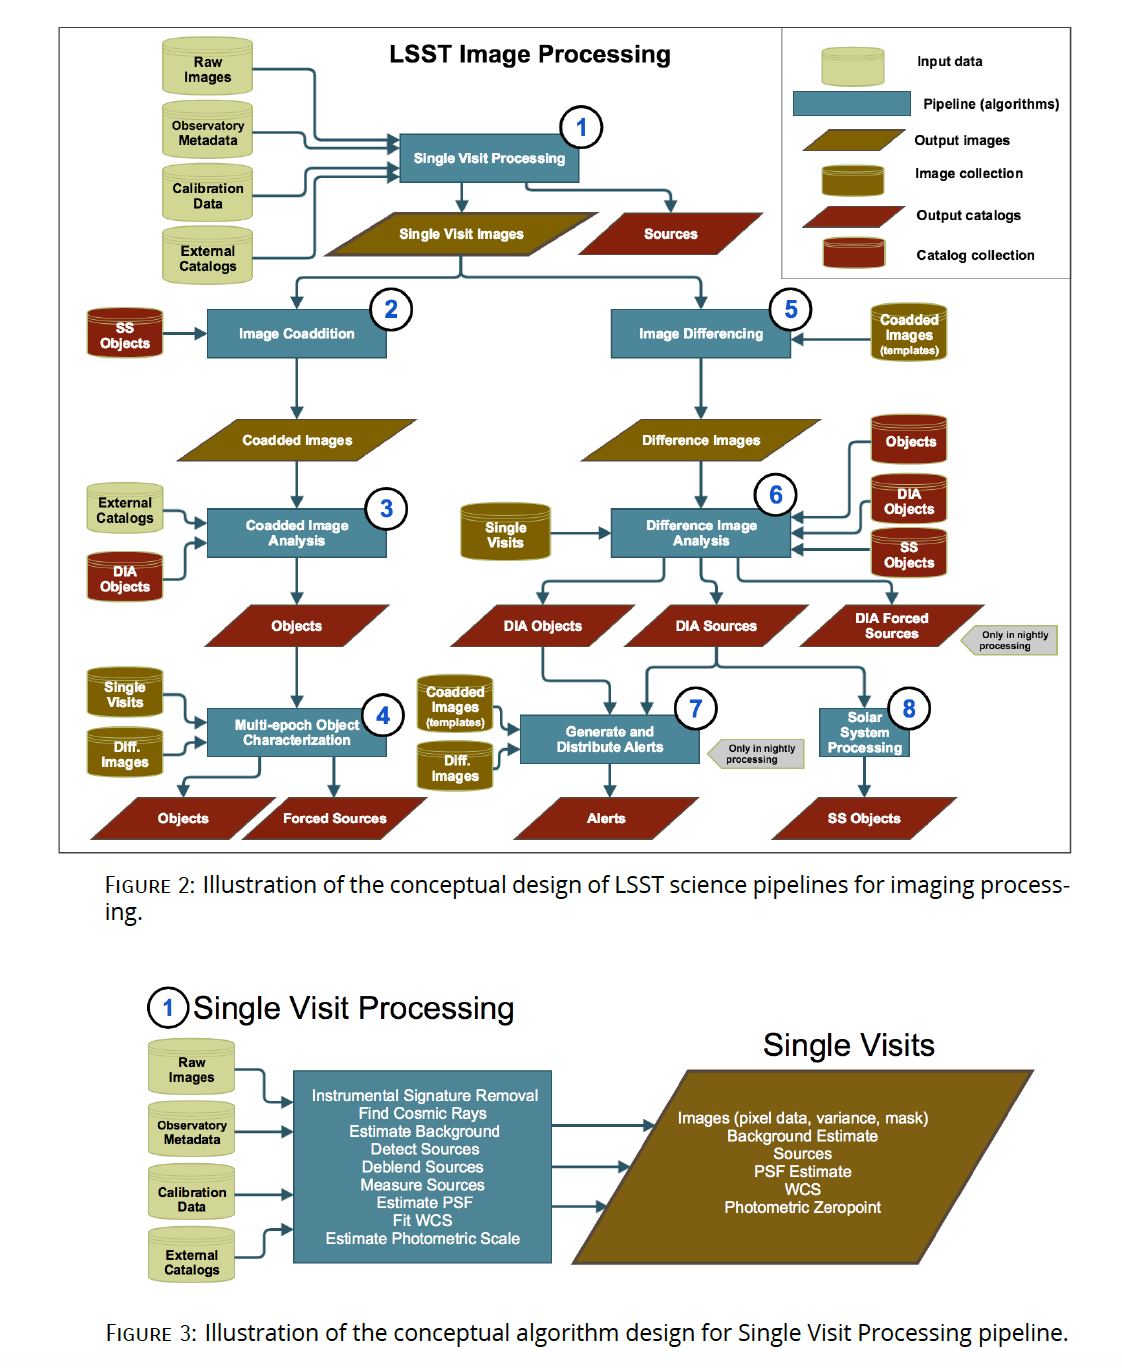
\includegraphics[width=12cm, height=12cm]{figs/dm/DMpipelines1.png}
\end{frame}

\begin{frame}{Rubin-LSST science pipeline}
\begin{tabular}{cc}
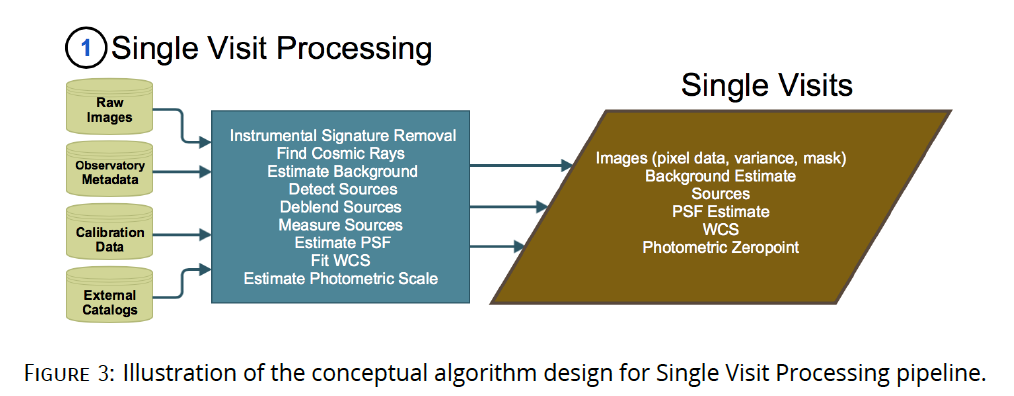
\includegraphics[width=6cm, height=3.5cm]{figs/dm/DMpipelines11.png}
&
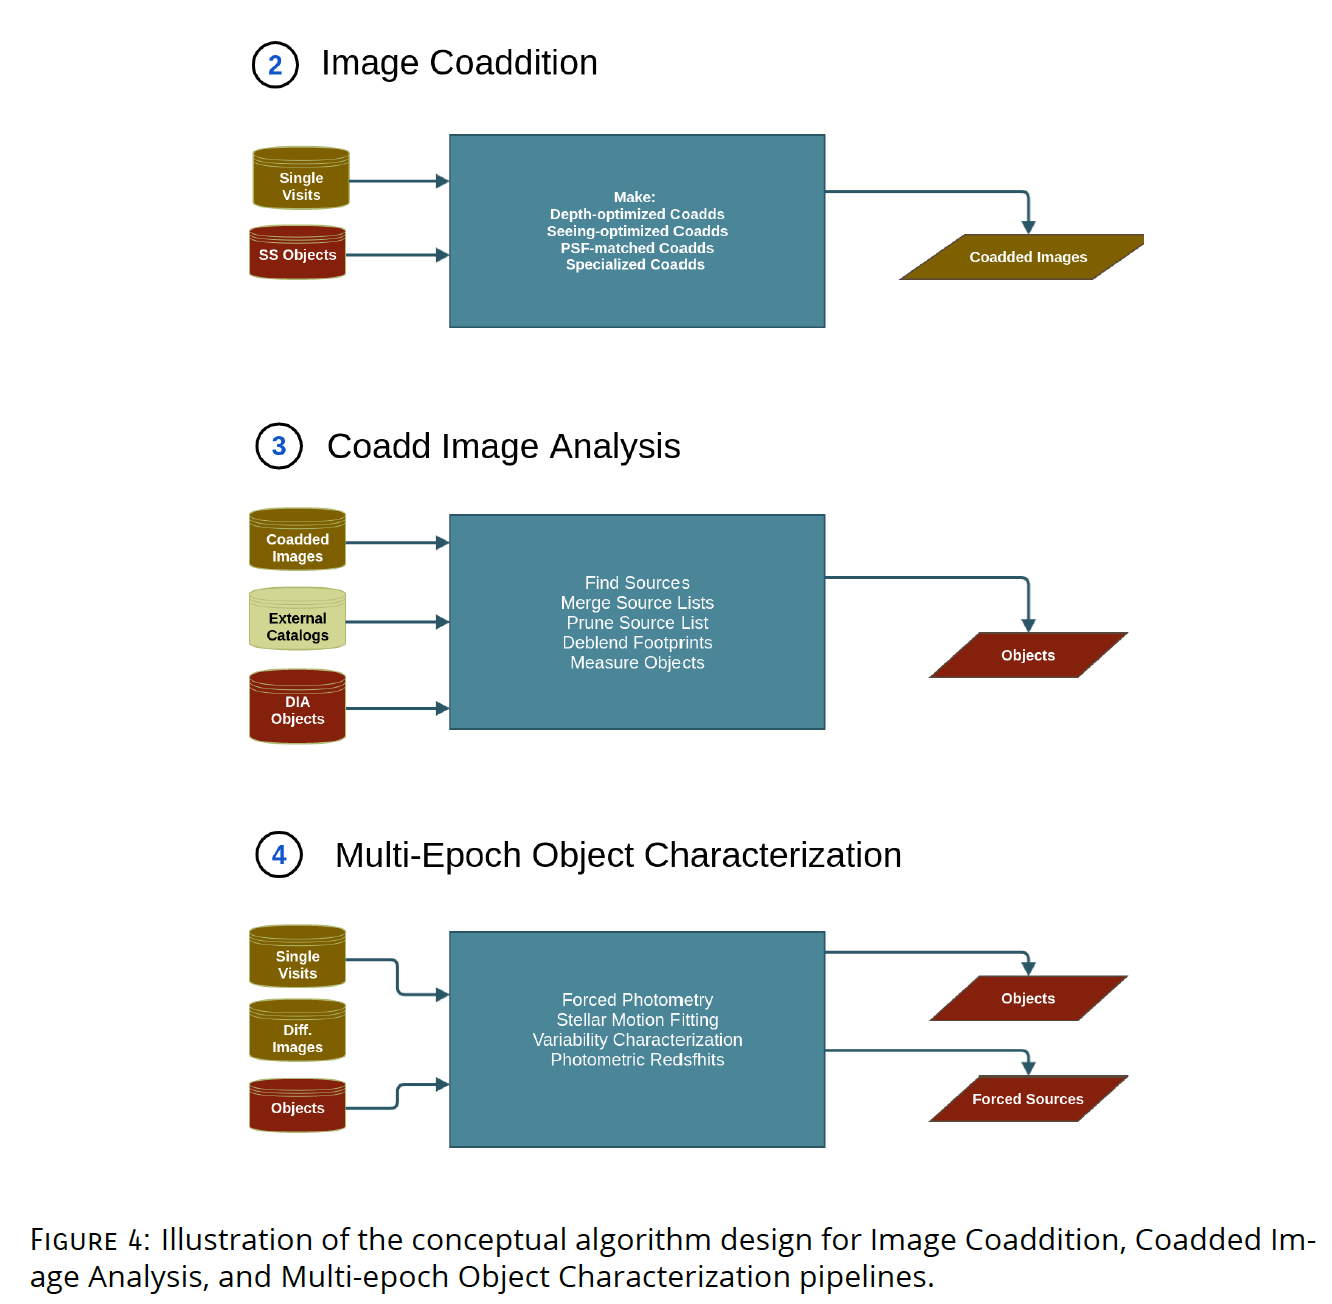
\includegraphics[width=6cm, height=8cm]{figs/dm/DMpipelines2.png}
\end{tabular}
\end{frame}

\begin{frame}{Rubin-LSST calibration plan}
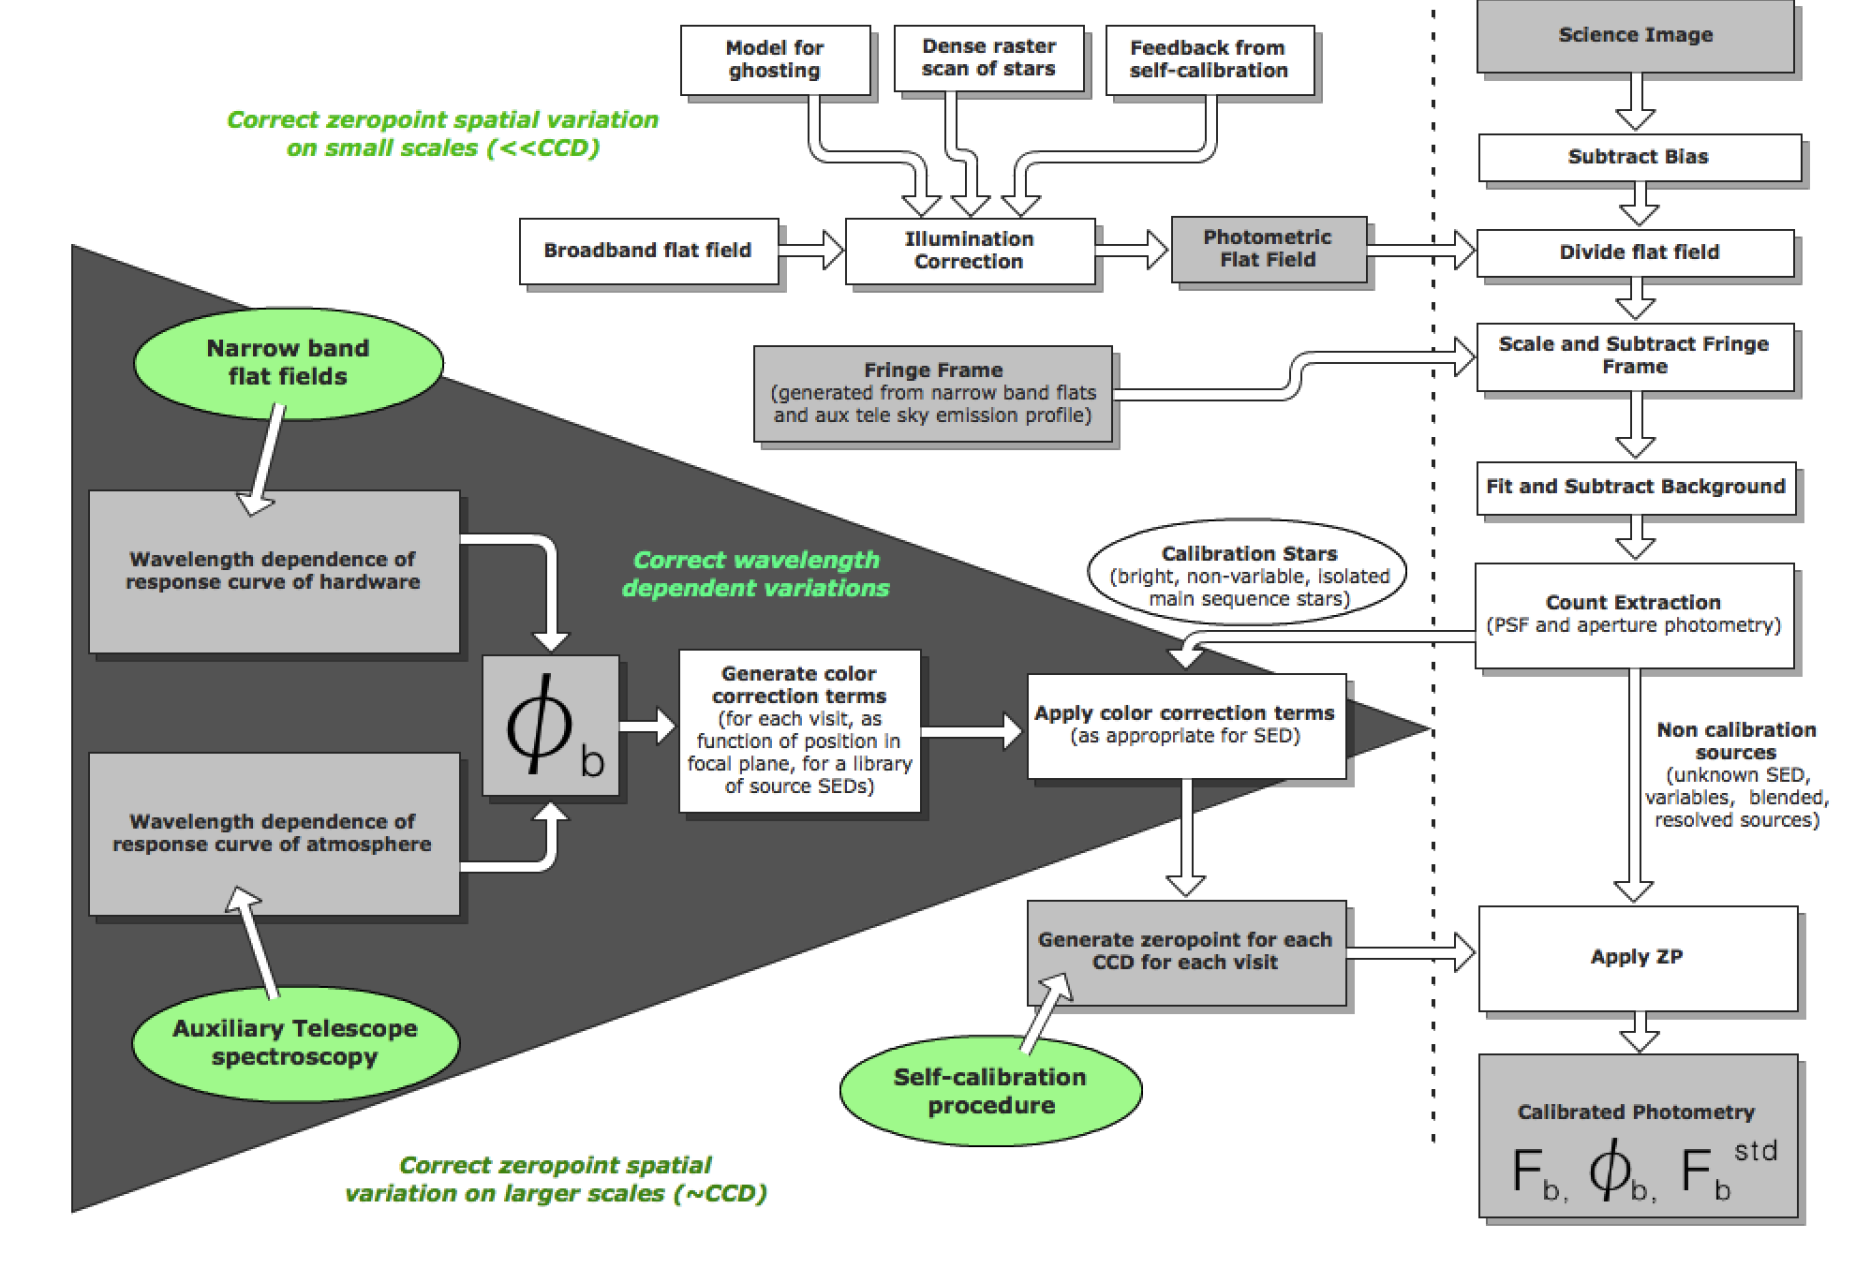
\includegraphics[width=12cm, height=8cm]{figs/calib/LSSTCalibrationPlan.png}
\end{frame}


\section{Simulation of the photometric corrections}

\subsection{Atmospheric simulation and $S_b^{obs}$}
%====================================================================
\begin{frame}{Atmospheric simulation and $S_b^{obs}$}
\begin{tabular}{cc}
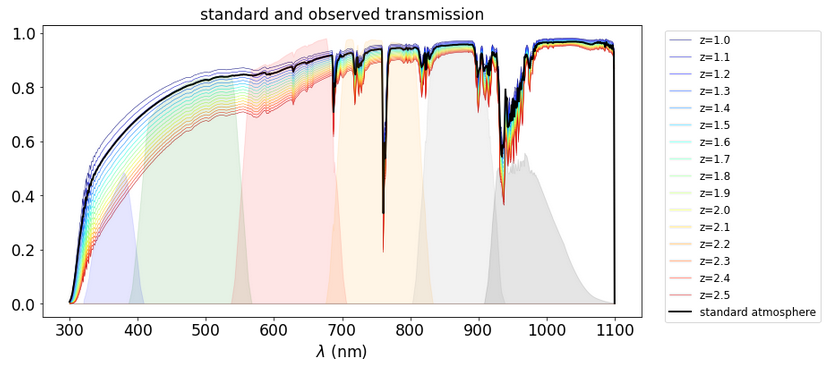
\includegraphics[width=5.9cm, height=3.5cm]{figs/atmsimu/atmsimvsairmass.png} & 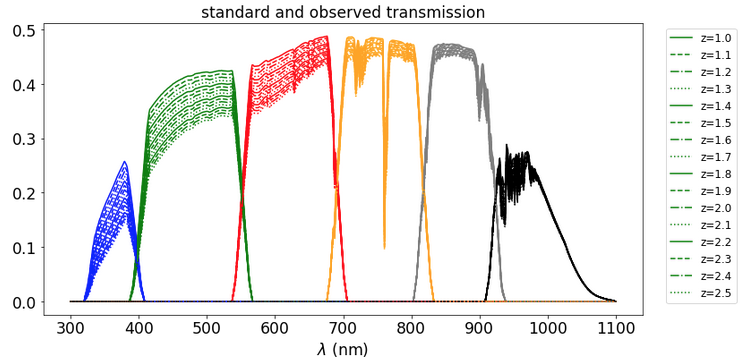
\includegraphics[width=5.9cm, height=3.5cm]{figs/atmsimu/trb_vs_airmass.png} \\
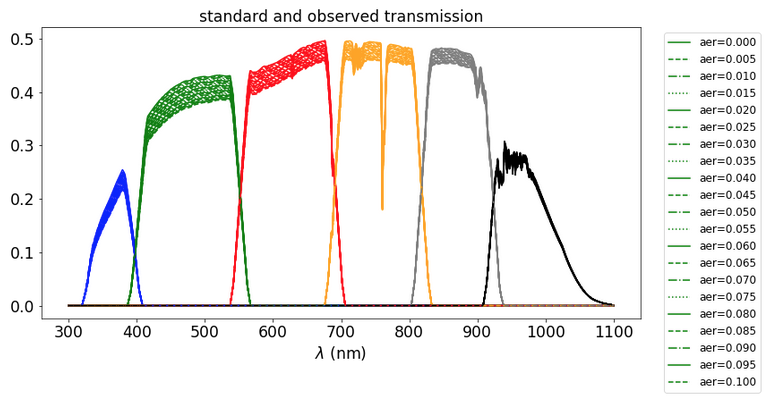
\includegraphics[width=5.9cm, height=3.5cm]{figs/atmsimu/trb_vs_VAOD.png} & 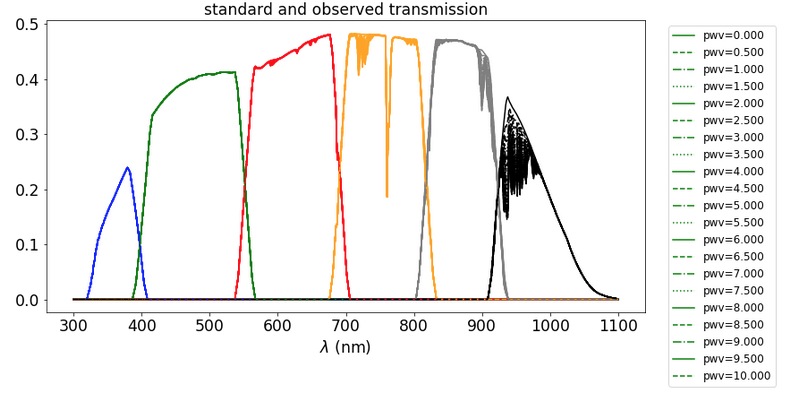
\includegraphics[width=5.9cm, height=3.5cm]{figs/atmsimu/trb_vs_PWV.png}
\end{tabular}
\end{frame}
%====================================================================


\subsection{The zero's order of the photometric correction}
%====================================================================
\begin{frame}{The $0^{th}$ order of the photometric correction}
\begin{alertblock}{vs airmass, relative to the standard transmission}
\begin{equation}
\mathbb{I}^{obs}_{0}(b,z) - \mathbb{I}^{std}_{0}(b,z_{std})
\end{equation}
\end{alertblock}
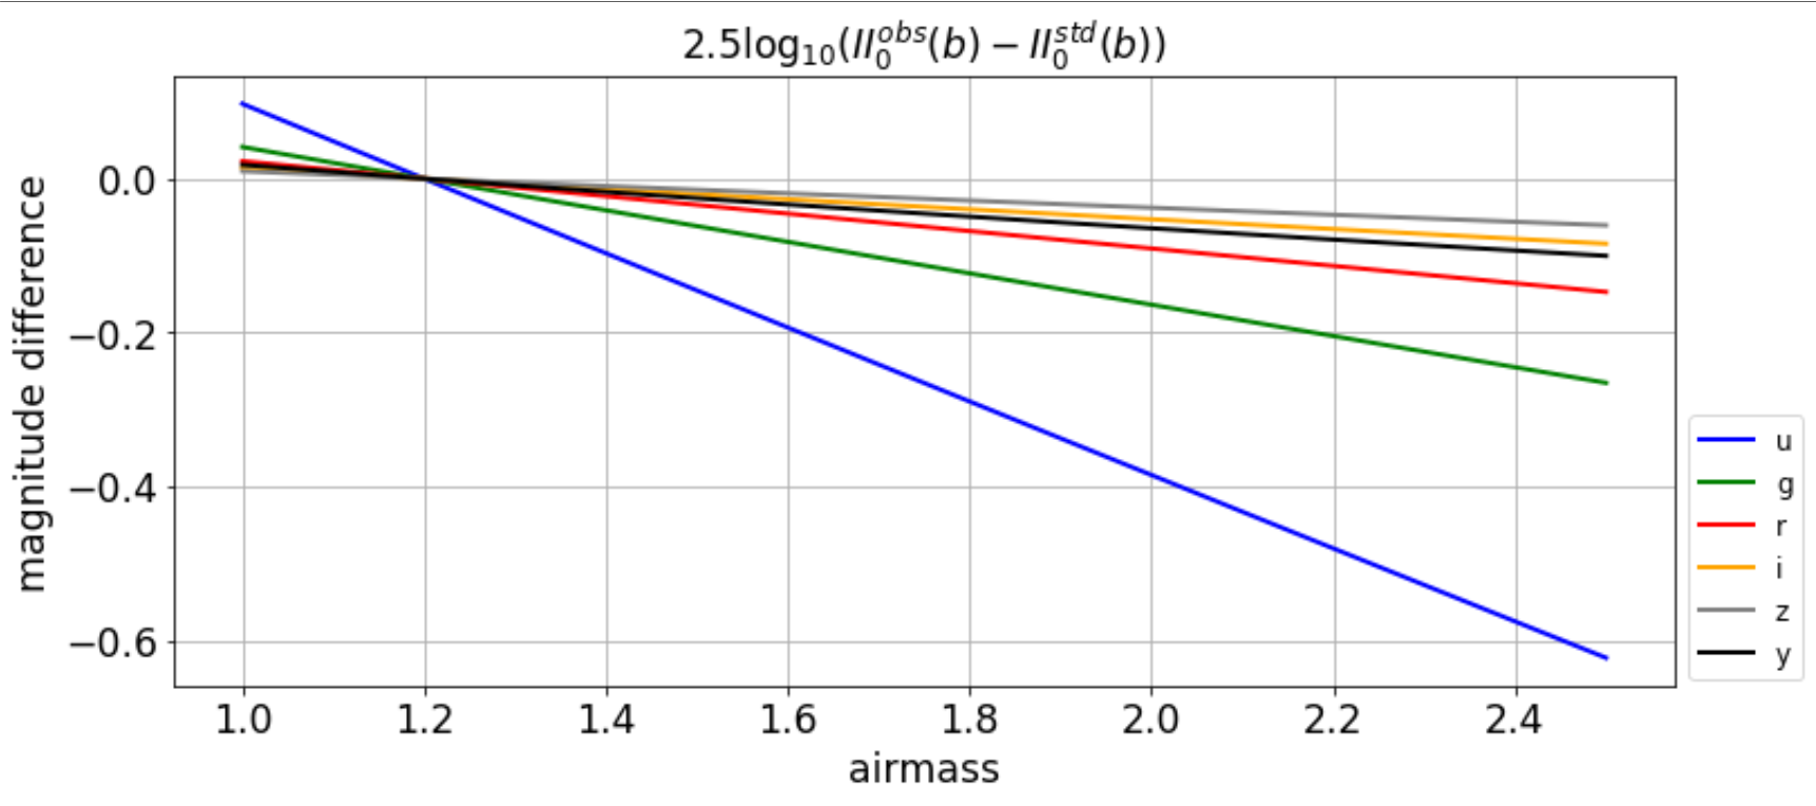
\includegraphics[width=10cm, height=5cm]{figs/Integrals_II/Integrals_II0_vs_airmass.png}
\end{frame}
%====================================================================


%====================================================================
\begin{frame}{The $0^{th}$ order of the photometric correction}
\begin{alertblock}{vs aeorols or PWV, relative to the standard transmission}
\begin{equation}
\mathbb{I}^{obs}_{0}(b,z_{std}) - \mathbb{I}^{std}_{0}(b,z_{std})
\end{equation}
\end{alertblock}
\begin{tabular}{cc}
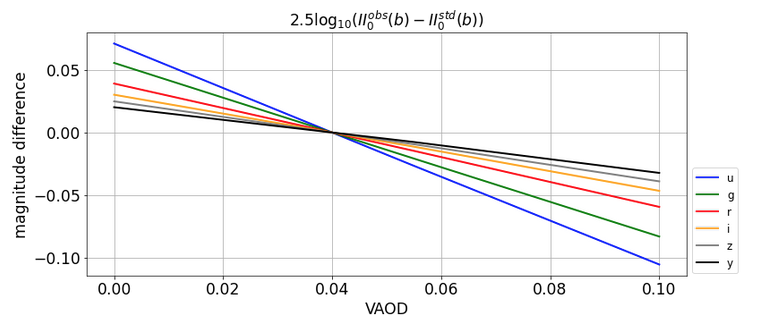
\includegraphics[width=5.9cm, height=4cm]{figs/Integrals_II/Integrals_II0_vs_VAOD.png} & 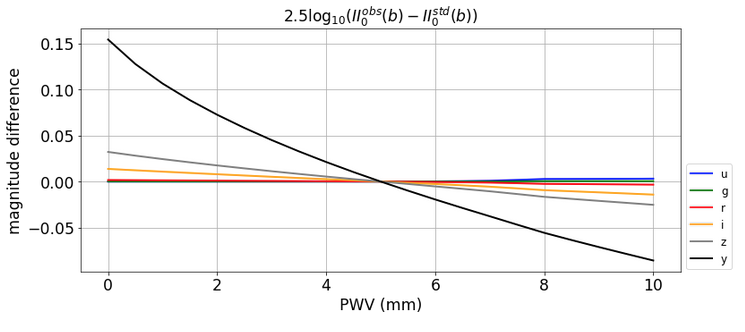
\includegraphics[width=5.9cm, height=4cm]{figs/Integrals_II/Integrals_II0_vs_PWV.png}
\end{tabular}
\end{frame}
%====================================================================

\subsection{The 1st and 2nd orders Integral differences}
%====================================================================
\begin{frame}{The $1^{st}$\&$2^{nd}$ orders Integral differences}

\begin{tabular}{cc}
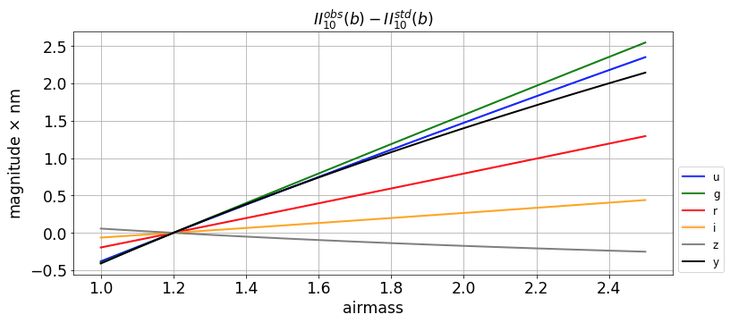
\includegraphics[width=5.9cm, height=4cm]{figs/Integrals_II/Integrals_II10_vs_airmass.png} & 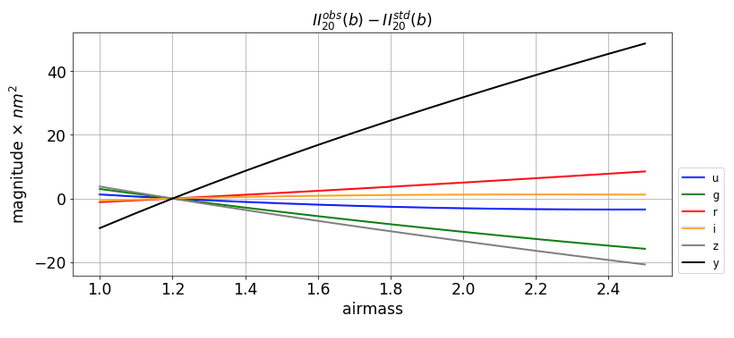
\includegraphics[width=5.9cm, height=4cm]{figs/Integrals_II/Integrals_II20_vs_airmass.png}
\end{tabular}
\end{frame}
%====================================================================


%==========================================================================================================================
\begin{frame}
\begin{center}
{\usebeamerfont{frametitle}

\LARGE \alert{End of part 1}}

\end{center}

\end{frame}
%==========================================================================================================================

 
\end{document}


